\documentclass[aspectratio=169]{beamer}

\usepackage{tikz}

\beamertemplatenavigationsymbolsempty%

\definecolor{sblau}{HTML}{007ec1}

\begin{document}

\begin{frame}
    \centering
    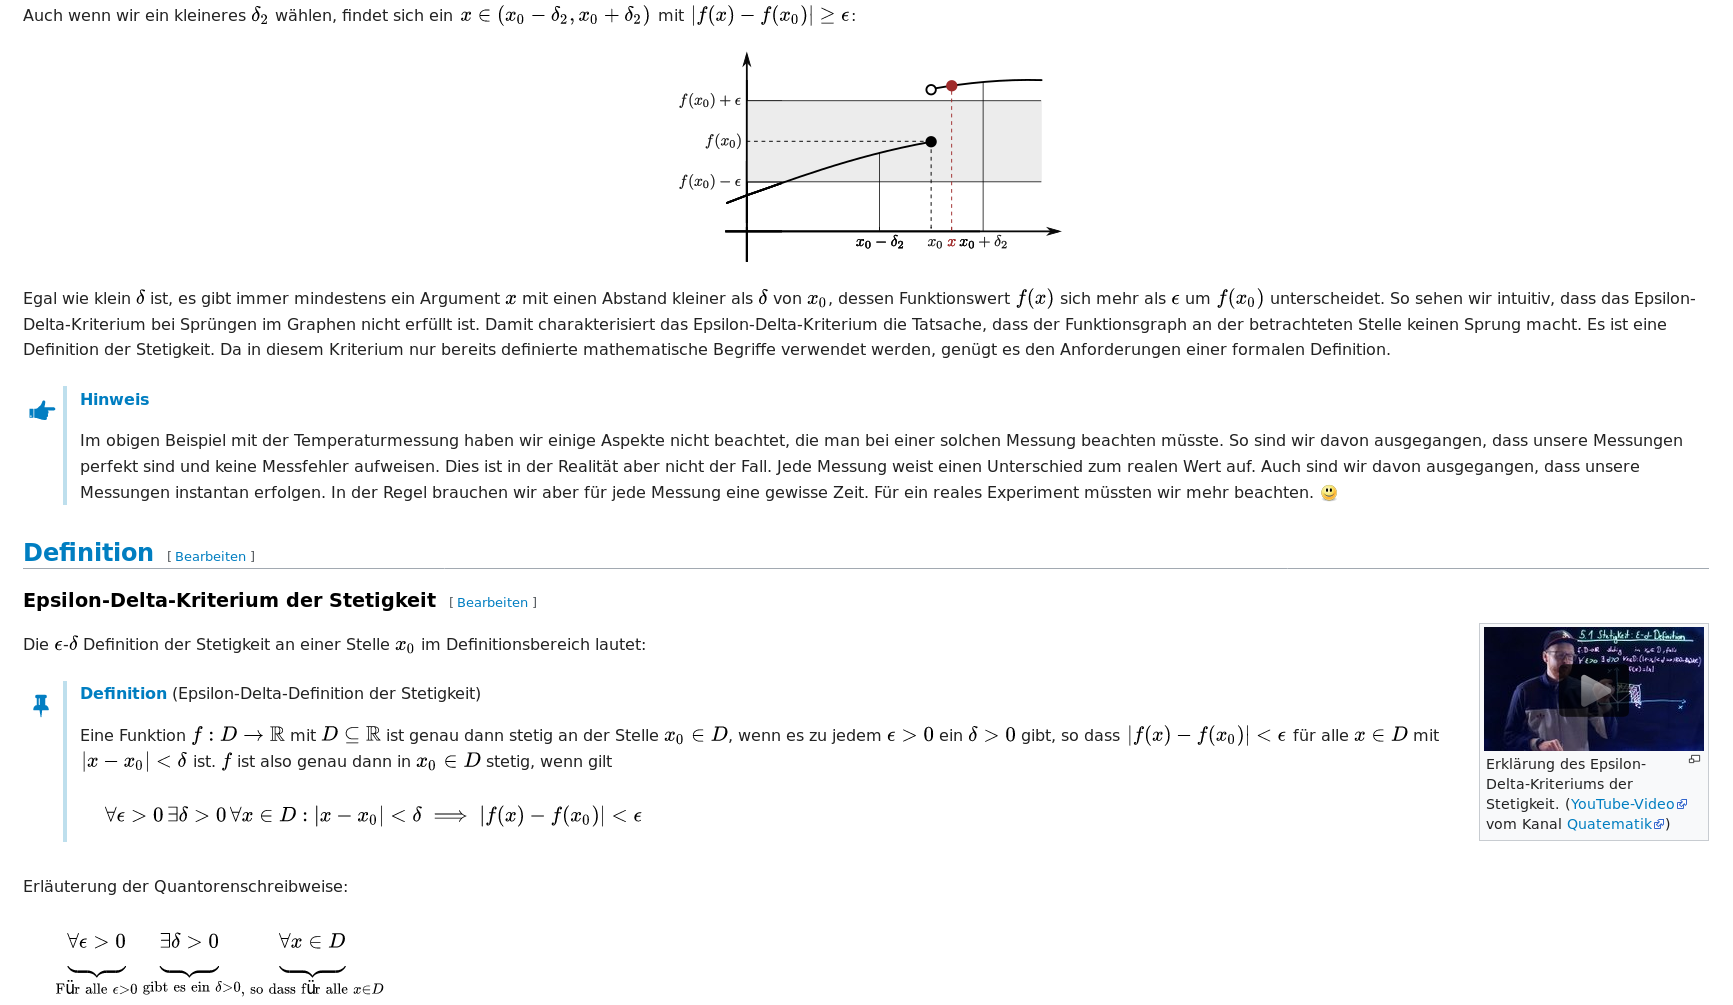
\includegraphics[height=0.9\textheight]{mfnf.png}
\end{frame}

\begingroup
\setbeamercolor{background canvas}{bg=sblau}
\begin{frame}
    \centering
    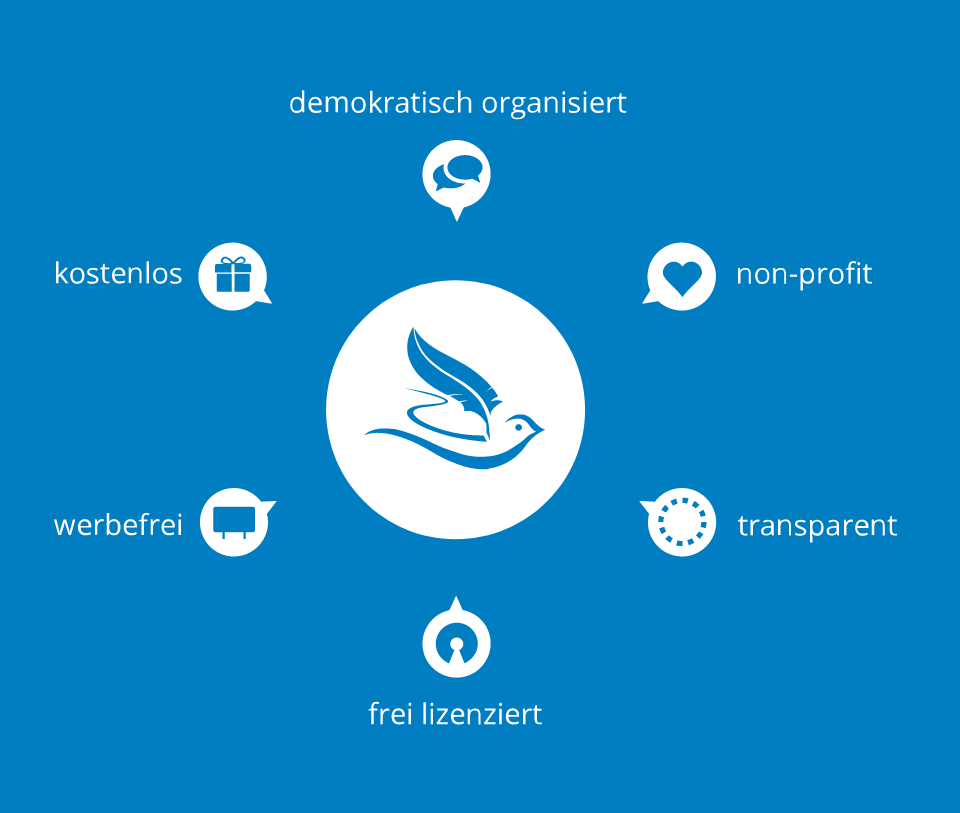
\includegraphics[height=\textheight]{serlo-vision.png}
\end{frame}
\endgroup

\begin{frame}
    \vfill

    \begin{minipage}[b]{0.3\textwidth}
        \centering
        
\includegraphics[width=3cm]{serlo-logo.png}
        \\[0.5em]
        783.934 Nutzer*innen\footnotemark[1]
    \end{minipage}
    \hfill
    \begin{minipage}[b]{0.3\textwidth}
        \centering
        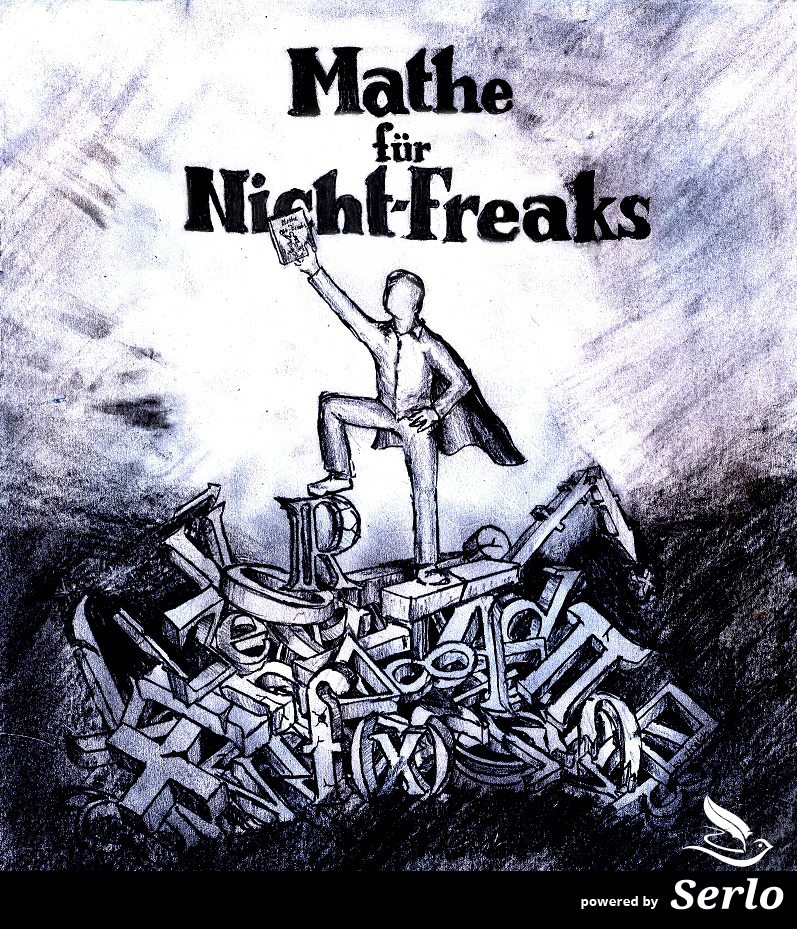
\includegraphics[width=3cm]{mfnf-logo.jpg}
        \\[0.5em]
        110.967 Nutzer*innen\footnotemark[1]
    \end{minipage}
    \hfill
    \begin{minipage}[b]{0.3\textwidth}
        \centering
        
\includegraphics[width=3cm]{serlo-abc-logo.png}
        \\[0.5em]
        500+ Installationen\footnotemark[1]
    \end{minipage}

    \begin{center}
        9300 Downloads \\ des PDF-Exports des Buchs Analysis 1
    \end{center}

    \footnotetext[1]{Pro Monat, Stand 2018}
\end{frame}

\begin{frame}
    \centering
    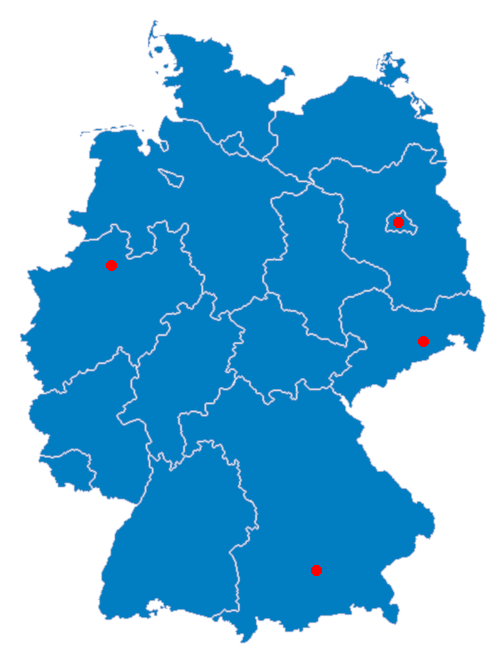
\includegraphics[height=0.8\textheight]{map.png}
    \begin{tikzpicture}[overlay]
        \node[anchor=east] (Berlin) at (3.8,4.65) {Berlin};
        \node[anchor=east] (Dresden) at (3.8,3.34) {Dresden};
        \node[anchor=east] (Munchen) at (3.8,0.83) {München};
        \node[align=left] (Munster) at (-9,4.18) {Münster};
        \draw[color=red] (Berlin.west) to (-1.26,4.65);
        \draw[color=red] (Dresden.west) to (-0.96,3.34);
        \draw[color=red] (Munchen.west) to (-2.2,0.83);
        \draw[color=red] (Munster.east) to (-4.4,4.18);
    \end{tikzpicture}
\end{frame}

\end{document}
